\documentclass{ximera}
\input{../preamble.tex}

\title{Challenge Problems for Ch 1} \license{CC BY-NC-SA 4.0}

\begin{document}

\begin{abstract}
\end{abstract}
\maketitle

\section*{Challenge Problems for Chapter 1}

\begin{problem}\label{prb:pills}
A man is ordered by his doctor to take $5$ units of vitamin A, $13$ units of vitamin B, and $23$ units of vitamin C each day. Three brands of vitamin pills are available, and the number of units of each vitamin per pill are shown in the accompanying table.

$$
\begin{array}{cccc}
\hline
		\textbf{Brand} &  \textbf{A} & \textbf{B} & \textbf{C} \\ \hline
		\textbf{1} & 1 & 2 & 4 \\
		\textbf{2} & 1 & 1 & 3 \\
		\textbf{3} & 0 & 1 & 1 \\ \hline
 \end{array}
$$

\begin{enumerate}
\item Find all combinations of pills that provide exactly the required amount of vitamins (no partial pills allowed).

\item If brands 1, 2, and 3 cost 3 cents, 2 cents, and 5 cents \ per pill, respectively, find the least expensive treatment.

$\answer{5}$ of brand 1, $\answer{0}$ of brand 2, $\answer{3}$ of brand 3

\end{enumerate}
\end{problem}

\begin{problem}\label{prb:tables}
A restaurant owner plans to use $x$ tables seating $4$, $y$ tables seating $6$, and $z$ tables seating $8$, for a total of $20$ tables. When fully occupied, the tables seat $108$ customers. If only half of the $x$ tables, half of the $y$ tables, and one-fourth of the $z$ tables are used, each fully occupied, then $46$ customers will be seated. Find $x$, $y$, and $z$.
\end{problem}

\begin{problem}\label{prb:2.43} The steady state temperature, $u$, of a plate solves Laplace's
equation, $\Delta u=0.$ One way to approximate the solution is to divide the plate into a square mesh and require the temperature
at each node to equal the average of the temperature at the four adjacent
nodes. In the following picture, the numbers represent the observed
temperature at the indicated nodes. Find the temperature at
the interior nodes, indicated by $x,y,z,$ and $w$. One of the equations is
$z=\frac{1}{4}\left( 10+0+w+x\right) $.

\begin{center}
   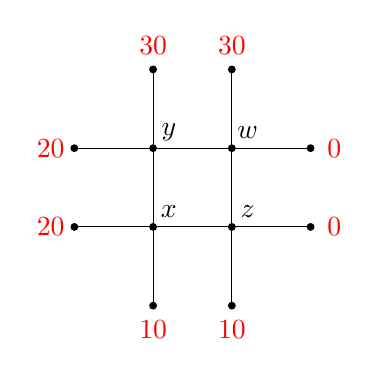
\begin{tikzpicture}[scale=1]
\node[red] at (-0.3, 1)   (a) {$20$};
\node[red] at (-0.3, 2)   (a) {$20$};
    \node[red] at (3.3, 1)   (b) {$0$};
     \node[red] at (3.3, 2)   (b) {$0$};
     \node[red] at (1, -0.3)   (c) {$10$};
      \node[red] at (2, -0.3)   (c) {$10$};
      \node[red] at (1, 3.3)   (c) {$30$};
      \node[red] at (2, 3.3)   (c) {$30$};
      \node[] at (1.2, 1.2)   (c) {$x$};
      \node[] at (2.2, 1.2)   (c) {$z$};
      \node[] at (1.2, 2.2)   (c) {$y$};
      \node[] at (2.2, 2.2)   (c) {$w$};
  \draw[-] (0,2)--(3,2);
  \draw[-] (0,1)--(3,1);
  \draw[-] (1,0)--(1,3);
  \draw[-] (2,0)--(2,3);
  \fill[] (1,1) circle (0.05cm); 
  \fill[] (1,2) circle (0.05cm); 
   \fill[] (2,1) circle (0.05cm); 
  \fill[] (2,2) circle (0.05cm); 
   \fill[] (0,1) circle (0.05cm); 
  \fill[] (0,2) circle (0.05cm); 
   \fill[] (3,1) circle (0.05cm); 
  \fill[] (3,2) circle (0.05cm); 
   \fill[] (1,0) circle (0.05cm); 
  \fill[] (1,3) circle (0.05cm); 
   \fill[] (2,0) circle (0.05cm); 
  \fill[] (2,3) circle (0.05cm); 
    \end{tikzpicture}
\end{center}

\begin{hint}
You need 
\begin{align*}
&\frac{1}{4}\left( 20+30+w+x\right) -y=0 \\
&\frac{1}{4}\left( y+30+0+z\right) -w=0 \\
&\frac{1}{4}\left( 20+y+z+10\right) -x=0 \\
&\frac{1}{4}\left( x+w+0+10\right) -z=0
\end{align*}
\end{hint}
 \begin{align*}
 w&=\answer{15}\\
 x&=\answer{15}\\
 y&=\answer{20}\\
 z&=\answer{10}\\
 \end{align*}
\end{problem}

\begin{problem}\label{prb:quadratic}
Solve the following system of equations for $x$ and $y$.

\begin{equation*}
\begin{array}{rlrlrcr}
	  x^2 & + &   xy & - &   y^2 & = &  1 \\
	 2x^2 & - &   xy & + &  3y^2 & = & 13 \\
	  x^2 & + &  3xy & + &  2y^2 & = &  0 \\
\end{array}
\end{equation*}

\begin{hint}
These equations are linear in the new variables $x_{1} = x^{2}$, $x_{2} = xy$, and $x_{3} = y^{2}$.
\end{hint}
\end{problem}

\begin{problem}\label{prob:parabolaFit}
    Find coefficients $a$, $b$ and $c$ such that the graph of $y=ax^2+bx+c$ passes through the points $(-2, 1)$, $(2, 5)$, $(4, 1)$.  Graph the equation you found to check your answer.  Given any three points in the plane, does a solution always exist?  What are the possibilities when only two points are given?  What about more than three points?  Illustrate your answers with examples.
\end{problem}

\begin{problem}\label{prob:lineFit}
    Use the concepts from Problem \ref{prob:parabolaFit} to establish the fact that two distinct points determine a line.
\end{problem}

\begin{problem}\label{prob:circleFit}
    A circle with radius $r$, centered at the origin is a graph of $x^2+y^2-r^2=0$.  How many points does it take to uniquely determine a circle with this equation?  In general, a circle is a graph of $x^2+y^2+ax+by+c=0$.  How many points determine a circle?  Can a circle be drawn through \emph{any} three points?  Support your answers geometrically and algebraically.
\end{problem}


\section*{Bibliography}
These problems come from the end of Chapter 1 of Ken Kuttler's \href{https://open.umn.edu/opentextbooks/textbooks/a-first-course-in-linear-algebra-2017}{\it A First Course in Linear Algebra}. (CC-BY)

Ken Kuttler, {\it  A First Course in Linear Algebra}, Lyryx 2017, Open Edition, pp. 42--49. 

\end{document}